\section{Komplexe Zahlen}

\subsection{Darstellungsformen von komplexen Zahlen}

\subsubsection{Normalform (kartesisch)} 

\vspace{-0.2cm}

$$ z = z_1 + \, \jimg z_2 \qquad z_1 = \RE(z) \qquad z_2 = \IM(z) \qquad \vert z \vert = \sqrt{z_1^2 + z_2^2} $$
\vspace{-2em}

$$ \RE(z) = \frac{1}{2}(z+\overline{z}) \qquad \qquad \IM(z) = \frac{1}{2\jimg}(z - \overline{z})$$

\para{Umrechnung in Polarform ($r, \varphi$)} 

\vspace{-0.2cm}

$$ r =  \vert z \vert = \sqrt{z_1^2 + z_2^2} \qquad 
\varphi = \begin{cases} 
\arctan\left(\frac{z_2}{z_1}\right), & z_1 > 0 \\ 
\arctan\left(\frac{z_2}{z_1}\right) + \pi, & z_1 < 0 
\end{cases} = \begin{cases} 
\arccos\left(\frac{z_1}{r}\right), & z_2 \geq 0 \\ 
-\arccos\left(\frac{z_1}{r}\right), & z_2 < 0 
\end{cases}$$


\subsubsection{Polarform / \cbl{Eulerform}}

\vspace{-0.2cm}

$$ z = r \cdot \cjs(\varphi) = r \cdot \left(\cos(\varphi) + \jimg \sin(\varphi)\right) = \cbl{r \cdot \e^{ \jimg \varphi}} \qquad \varphi = \arg(z) $$


\para{Umrechnung in Normalform (kartesisch)}\vspace{-0.2cm}

$$ \RE(z) = z_1 = \vert z \vert \cdot \cos(\varphi) \qquad \qquad \IM(z) = z_2 = \vert z \vert \cdot \sin(\varphi) $$ 

\subsubsection{Wichtige Zusammenhänge}\vspace{-0.5cm}

\[\jimg^2 = -1 \qquad \frac{1}{\jimg} = -\jimg \qquad \e^{\jimg \, \pi} = -1 \qquad
\e^{\jimg \frac{\pi}{2}} = \jimg \qquad \jimg^{\jimg} = \e^{- \frac{\pi}{2} + 2k \pi} \qquad | \cjs(\varphi)| = 1 \]

\[e^{\jimg \varphi} = \cjs(\varphi) \qquad \cjs(\alpha) \cdot \cjs(\beta) = \cjs(\alpha + \beta) \qquad \cjs(\alpha) : \cjs(\beta) = \cjs(\alpha - \beta)\]

$$z_1 \perp z_2 \Leftrightarrow \RE\left(\frac{z_1}{z_2}\right) = 0 \Leftrightarrow \arg\left(\frac{z_1}{z_2}\right) = \pm \frac{\pi}{2}$$

\subsubsection{Geometrische Aspekte von komplexen Zahlen}

\begin{minipage}[t]{0.47\columnwidth}
    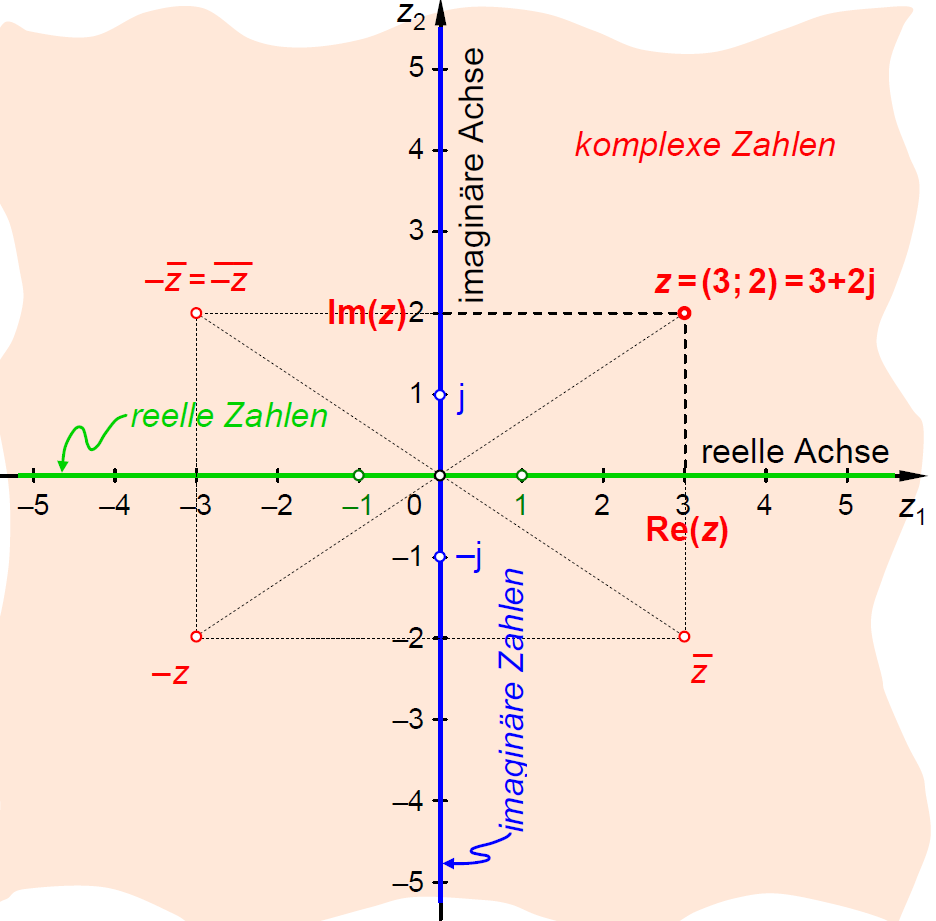
\includegraphics[width=\linewidth, align=t]{images/komplexe_zahlen_uebersicht.png}
\end{minipage}
\hfill
\begin{minipage}[t]{0.47\columnwidth}
    \para{komplex-konjugieren}

    \textrightarrow\ Spiegelung an \textbf{reeller} Achse

    $$z = 3 + 2\jimg \quad \rightarrow \quad \overline{z} = 3 - 2\jimg$$
    \vspace{1em}

    \renewcommand{\arraystretch}{1.5}
    \begin{tabular}{l c l}
        $\overline{a + b} = \overline{a} + \overline{b}$            & & $\overline{a - b} = \overline{a} - \overline{b}$          \\ 
        $\overline{a \cdot b} = \overline{a} \cdot \overline{b}$    & & $\overline{a \div b} = \overline{a} \div \overline{b}$
    \end{tabular}
    \renewcommand{\arraystretch}{1}

    \medskip
    \medskip

    \para{Multiplikation mit $\bm{(-1)}$}

    \textrightarrow\ Punktspeigelung am Ursprung

\end{minipage}


\subsection{Rechenoperationen}

\subsubsection{Addition / Subtraktion}

Gleiches Vorgehen wie in $\mathbb{R}$ (\textbf{kartesisch})

\smallskip

\renewcommand{\arraystretch}{1.4}
\begin{tabular}{ll}
    Addition:       & $(a_1 + \jimg a_2) + (b_1 + \jimg b_2) = (a_1 + b_1) + \jimg (a_2 + b_2)$ \\
    Subtraktion:    & $(a_1 + \jimg a_2) - (b_1 + \jimg b_2) = (a_1 - b_1) + \jimg (a_2 - b_2)$ 
\end{tabular}
\renewcommand{\arraystretch}{1}


\subsubsection{Multiplikation}

\renewcommand{\arraystretch}{1.4}
\begin{tabular}{ll}
    kartesisch:     & $(a_1 + \jimg a_2) \cdot (b_1 + \jimg b_2) = (a_1 b_1 - a_2 b_2) + \jimg (a_1 b_2 + a_2 b_1)$ \\
    \textbf{polar:} & $a \cdot b = \vert a \vert \vert b \vert \, e^{\jimg (\varphi_1 + \varphi_2)}$                \\
                    & \textrightarrow\ Beträge multiplizieren und Argumente (Winkel) addieren
\end{tabular}
\renewcommand{\arraystretch}{1}

La moltiplicazione equivale ad una rotazione di angolo $\arg(b)$ e una streckung di $\vert b \vert$.

\subsubsection{Division}

\renewcommand{\arraystretch}{1.6}
\begin{tabular}{ll}
    kartesisch:     & $\frac{(a_1 + \jimg a_2)}{(b_1 + \jimg b_2)} = 
                    \frac{(a_1 + \jimg a_2) \cbl{(b_1 - \jimg b_2)}}{(b_1 + \jimg b_2) 
                    \cbl{(b_1 - \jimg b_2)}} = \frac{\text{ausmultiplizieren}}{b_1^2 + b_2^2}$ 
                    \qquad {\small$\color{blue}\blacksquare$: Konjugiert komplexe}\\
    \textbf{polar:} & $\frac{a}{b} = \frac{\vert a \vert}{\vert b \vert} \, \e^{\jimg (\varphi_1 - \varphi_2)}$                                                                                                    \\
                    & \textrightarrow\ Beträge dividieren und Argumente (Winkel) subrahieren
\end{tabular}
\renewcommand{\arraystretch}{1}

\smallskip

\textbf{Hinweis:} Es gilt: $\Big| \frac{a}{b} \Big| = \frac{\vert a \vert}{\vert b \vert}$ 


\subsubsection{Potenzieren (De Moivre)}

\textbf{Potenzgesetze gelten weiterhin für \myul{ganzzahlige} Exponenten!}

\[z^n = r^n \cdot \big[ \cos(\alpha) + \jimg \sin(\alpha) \big]^n = r^n \cdot \big[ \cos(n \alpha) + \jimg \sin(n \alpha) \big] \qquad \text{ für } n \in \mathbb{N} \]

Mit der Formel von de Moivre können \textbf{Mehrfachwinkelformeln} aus der Trigo hergleitet
werden:\vspace{-1em}

\begin{center}
    \begin{tabular}{cl}
        $\underbrace{[\cos(\zeta) + \jimg \sin(\zeta)]^2} $ & $= {\color{green}\cos(2\zeta)} + \jimg {\color{blue}\sin(2\zeta)}$ \\
        $= [\cos(\zeta)]^2 + 2\jimg \cos(\zeta)\sin(\zeta) + \jimg^2 [\sin(\zeta)]^2$ &\\
        $= [{\color{green}\cos(\zeta)}]^2 - [{\color{green}\sin(\zeta)}]^2 + \jimg \cdot {\color{blue}2 \sin(\zeta) \cos(\zeta)} $&
    \end{tabular}
\end{center}

% 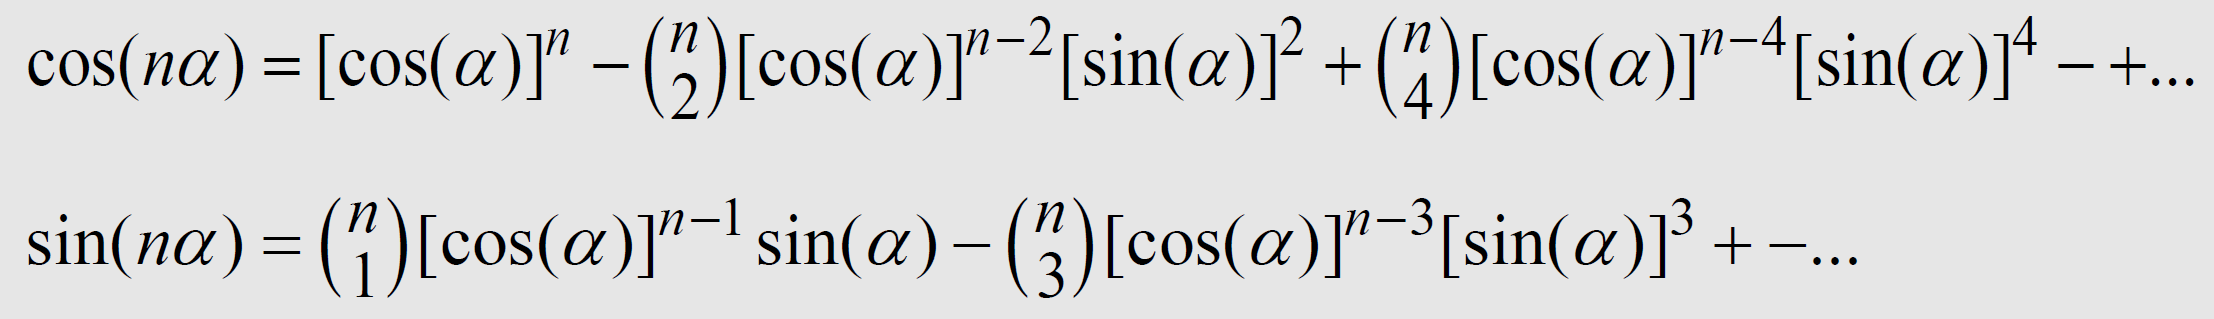
\includegraphics[width=\columnwidth]{images/mehrfachwinkel_2.PNG}
\subsubsection{Estrazione di radice $n$-esima (Radicazione)}

\begin{itemize}
    \item \textbf{Proprietà:} Le distributive delle radici \textbf{non si estendono} generalmente al campo complesso ($\sqrt{ab} \neq \sqrt{a}\sqrt{b}$ in $\mathbb{C}$).
    \item \textbf{Molteplicità:} Ogni numero complesso $a \neq 0$ ammette esattamente $n$ radici $n$-esime distinte in $\mathbb{C}$.
    \item \textbf{Geometria:} Le soluzioni si dispongono nel piano come i vertici di un \textbf{$n$-agono regolare} centrato nell'origine e inscritto in una circonferenza di raggio $R = \sqrt[n]{|a|}$.
\end{itemize}\vspace{-0.8em}

\[z^n = a \implies z_k = \sqrt[n]{|a|} \left( \cos \frac{\varphi + 2k\pi}{n} + \jimg \sin \frac{\varphi + 2k\pi}{n} \right), \quad k \in \{0, 1, \dots, n-1\}\]\vspace{-0.5em}
% \[z^n = a  \qquad \vert z \vert = \sqrt[n]{\vert a \vert} \qquad \qquad \arg(z_1) = \frac{\arg(a)}{n} \qquad \arg(z_n) = \frac{\arg(a)}{n}+k\cdot \frac{2\pi}{n}\]

\example{Determinazione delle radici quarte di $-16$ ($z^4 = -16$)}

\begin{minipage}{0.58\columnwidth}
    \begin{enumerate}
        \item \textbf{Modulo ($|z_k|$):}
        \begin{align*}
            \lvert z \rvert^4 \cdot \cjs(4 \varphi) &= 16 \cdot \cjs(\pi)\\
            z = \sqrt[4]{\lvert 16 \rvert} &= 2
        \end{align*}
        \item \textbf{Argomento principale ($z_0$):}
    
        Si divide l'argomento $\arg(a) = \pi$ per l'indice $n=4$:
        \begin{equation*}
            \alpha_0 = \frac{\arg(a)}{n} = \frac{\pi}{4} = 45^\circ
        \end{equation*}
        \item \textbf{Argomenti successivi:}
        Si applica un incremento angolare costante $\Delta\varphi = \frac{2\pi}{n} = \frac{\pi}{2}$:
        \begin{align*}
            \alpha_1 &= \frac{\pi}{4} + \frac{\pi}{2} = \frac{3\pi}{4} \\
            \alpha_2 &= \frac{3\pi}{4} + \frac{\pi}{2} = \frac{5\pi}{4} \\
            \alpha_3 &= \frac{5\pi}{4} + \frac{\pi}{2} = \frac{7\pi}{4}
        \end{align*}
    \end{enumerate}    
\end{minipage}
\hfill
\begin{minipage}{0.38\columnwidth}
    \centering
    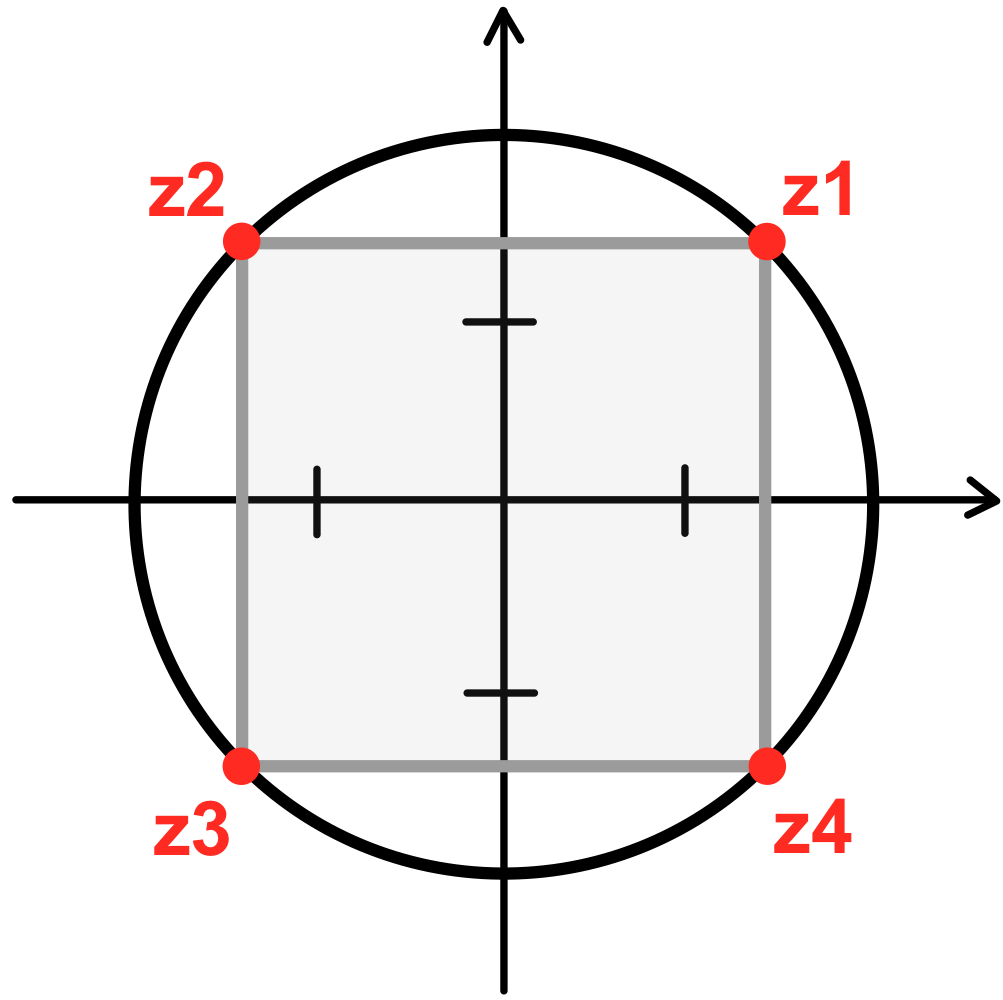
\includegraphics[width=\linewidth]{images/wurzel.png}
    \begin{align*}
        z_0 &= \sqrt{2} + \jimg\sqrt{2} \\
        z_1 &= -\sqrt{2} + \jimg\sqrt{2} \\
        z_2 &= -\sqrt{2} - \jimg\sqrt{2} \\
        z_3 &= \phantom{-}\sqrt{2} - \jimg\sqrt{2}
    \end{align*}
\end{minipage}

% Versione ottimizzata del formalismo di Steiner
Posto $a = r \mathrm{e}^{\jimg \varphi}$, l'insieme delle radici $n$-esime è definito come:
\begin{equation*}
    \mathcal{S} = \left\{ \sqrt[n]{r} \cdot \mathrm{e}^{\jimg \left( \frac{\varphi}{n} + \frac{2k\pi}{n} \right)} \;\middle|\; k \in \mathbb{Z}, \, 0 \le k < n \right\}
\end{equation*}
\para{Einheitswurzel $\bm{\sqrt[n]{1}}$}		

Durch Multiplikation mit der $n$-ten Einheitswurzel erreicht man eine reine Drehung um $\frac{360}{n}$ Grad im \textbf{Gegenuhrzeigersinn}. \\	
\textbf{Achtung!} Die erste Lösung von $\sqrt[n]{1}$ ist immer die reelle Zahl 1\\
\textrightarrow\ nächste Lösung verwenden!

\begin{center}
    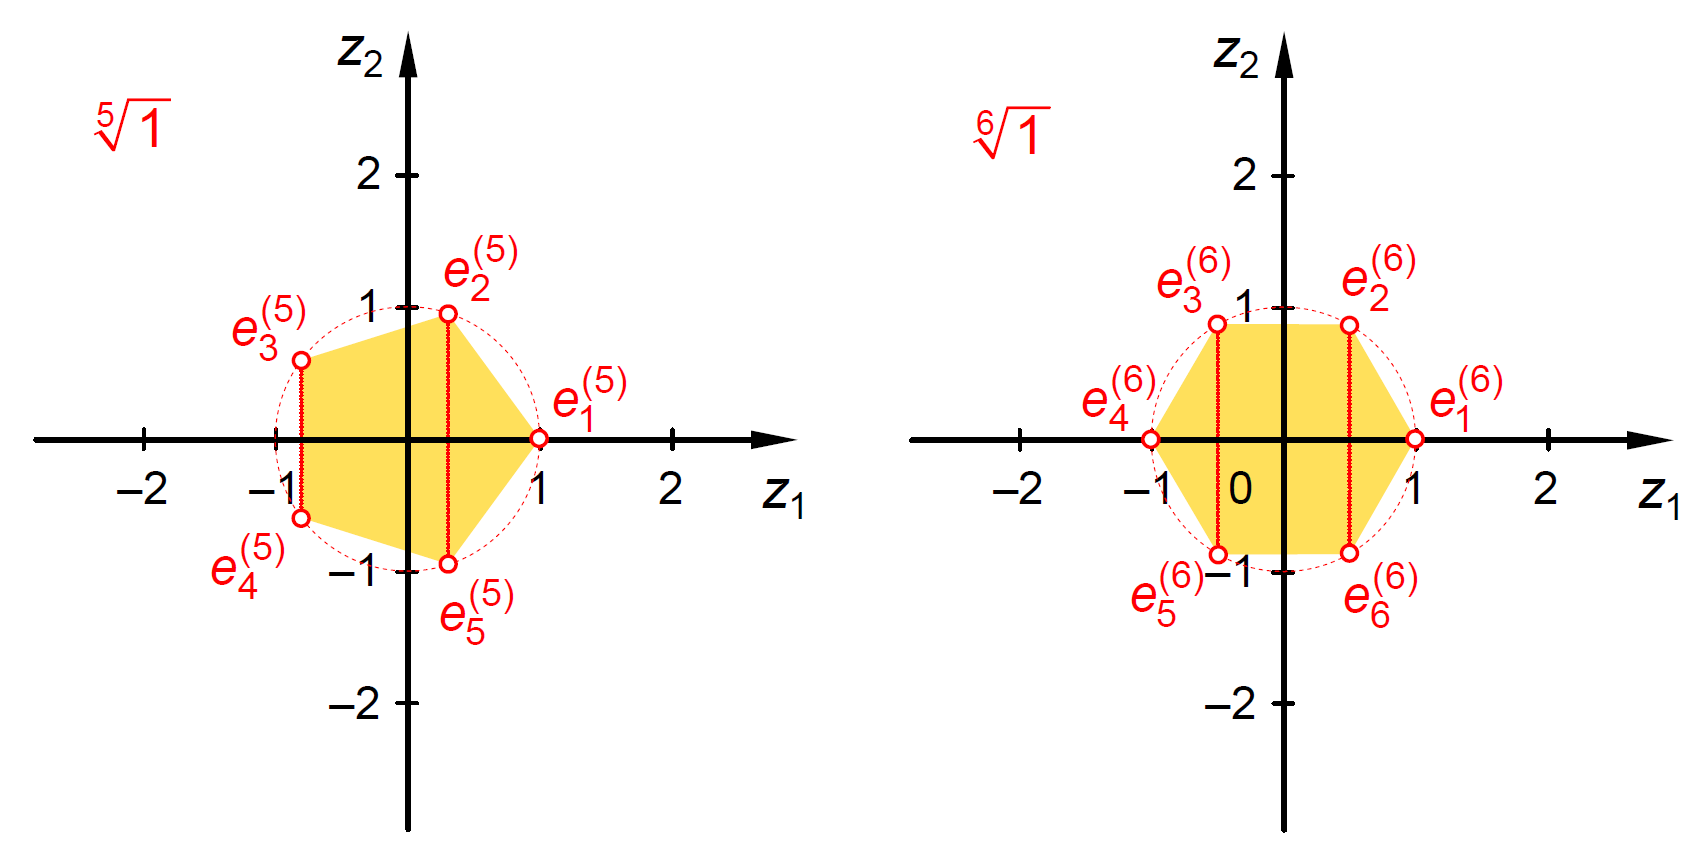
\includegraphics[width=0.9\columnwidth]{images/einheitswurzel.PNG}
\end{center}

\subsubsection{Komplexwertige Exponentialfunktion}

\vspace{-0.2cm}

\[\e^z = \e^{z_1 + \jimg z_2} = \e^{z_1} \cdot \e^{\jimg z_2} = \e^{z_1} \cdot \cjs(z_2) \qquad \rightarrow \qquad \boxed{e^{\jimg \varphi} = \cjs(\varphi)}\]

\textrightarrow\ Die Exponentialfunktion ist $2 \pi \jimg$-periodisch (auf imaginärer Achse)

\medskip

\para{Exponentialgesetze}

Die Exponentialgesetze bleiben in $\mathbb{C}$ für \myul{ganzzahlige} Exponenten erhalten!

\smallskip

\begin{tabular}{l c l c l}
    $\e^a \cdot \e^b = \e^{a+b}$    & & $\e^a : \e^b = \e^{a-b}$    & & $a, \; b \in \mathbb{C}$    \\
    $(\e^a)^k = \e^{ka}$            & &                             & & $k \in \mathbb{Z}$
\end{tabular}


\example{Exponentialfunktion}

\begin{itemize}
    \item $\e^z = e^{\cor{1}\cbl{-\frac{\pi}{2}} \jimg} = \e^{\cor{1}} \cdot \cjs(\cbl{- \frac{\pi}{2}}) = \e \cdot (- \jimg) = -2.781 \jimg$
    \item $\e^z = \e^{\cor{\ln(2)} + \cbl{3 \pi} \jimg} = \e^{\cor{\ln(2)}} \cdot \cjs(\cbl{3 \pi}) = 2 \cdot \cjs(\pi) = -2$ 
\end{itemize}



\subsubsection{Komplexwertige Logarithmusfunktion}

\textbf{\crd{Ehemalige Log-Gesetze sind nur noch Kongruenzgesetze!}}

\[ \Ln(z) = \ln(\vert z \vert) + \jimg (\arg(z)+ \cor{k2\pi}) \qquad (z \in \mathbb{C}, \, z \neq 0, k \in \mathbb{Z})\]

\textrightarrow\ Die Exponentialfunktion ist $\cor{2 \pi \jimg\text{-periodisch}}$ ($\infty$ viele lösungen)

    

\subsubsection{Allgemeine Potenzfunktion}

\textbf{\crd{Es existieren keine Potenz- oder Kongruenzgesetze!}} 
\[a^b = \e^{b \cdot \Ln(a)} \qquad (a, \; b \in \mathbb{C}, \; a \neq 0)\]


\subsubsection{Komplexwertige Trigonometrische Funktionen}

\vspace{-0.2cm}

\[\sin(\alpha \cdot z) = \frac{\e^{\alpha \jimg z} - \e^{-\alpha \jimg z}}{2 \jimg} \qquad 
\cos(\alpha \cdot z) = \frac{\e^{\alpha \jimg z} + \e^{-\alpha \jimg z}}{2} \qquad 
\tan(z) = \frac{\e^{\jimg z} - \e^{-\jimg z}}{\jimg(\e^{\jimg z} + \e^{-\jimg z})}\]


\subsection{Polynome (vgl. Radizieren)}
Alle Nullstellen des Polynoms $p(z) = a_n z^n + a_{n-1}z^{n-1} + \ldots + a_0$ liegen in der Gauss'schen Zahlenebene in einer
Kreisscheibe um den Ursprung mit Radius $\sum\limits _{k=0}^n \bigl| \frac{a_k}{a_n} \bigl|$

\smallskip

Für Gleichungen vom Grad $\geq$ 5 existieren \textbf{keine} nur aus den 4 Grundoperationen und Wurzeln zusammengesezten Lösungsformeln.	


\subsubsection{Polynome mit Koeffizienten $\bm{\in \mathbb{C}}$}

Wichtige Eigenschaften von komplexen \textbf{und} reellen Polynomen:

\smallskip

\begin{enumerate}[itemsep=0.2cm]
    \item Jedes komplexe Polynom vom Grad $\geq 1$ hat in $\mathbb{C}$ mindestens eine Nullstelle
    \item Ein komplexes Polynom vom Grad $n$ zerfällt in $\mathbb{C}$ in lauter Linearfaktoren. \\
        Die Faktoren müssen \textbf{nicht} verschieden sein.
        Die Zerlegung ist bis auf die Reihenfolge eindeutig. \\
        Beispiel: $a_n z^n + a_{n-1}z^{n-1} + \ldots + a_0 \quad \underrightarrow{\text{umformen}} \quad a_n \cdot (z - z_1) \cdot (z - z_2) \cdot \ldots \cdot (z - z_n)$
    \item Vielfachheit: Ein komplexes Polynom vom Grad $n$ hat in $\mathbb{C}$ \textbf{genau} $n$ (verschiedene) Nullstellen, wenn diese mit ihrer 
        Vielfachheit gezählt werden
\end{enumerate}

\medskip

\para{Determinazione del Vorfaktor $a_n$}

Per determinare il coefficiente principale \textbf{$a_n$}:
\begin{enumerate}
    \item \textbf{Dall'equazione:} È il coefficiente del termine con la potenza più alta ($z^n$).
    \item \textbf{Per sostituzione:} Se conosci le radici $z_i$ e un punto $P(z_0) = y_0$, allora:
    \[ a_n = \frac{y_0}{\prod_{i=1}^{n} (z_0 - z_i)} \]
\end{enumerate}

\medskip

\para{Tipps und Tricks für Lösung von $\bm{p(z) = 0}$}

\smallskip

\begin{ctabular}{ll}
    \toprule
    \textbf{Methode}    & \textbf{Beispiel für Anwendung}                                               \\
    \midrule
    Mitternachtsformel  & $p(z) = z^2 + (5 - 4 \jimg) z + (3 - 11 \jimg)$                               \\
    \midrule
    Wurzel ziehen       & $p(z) = z^3 -8 \jimg \quad \Leftrightarrow \quad z^3 = 8 \jimg$               \\
    \midrule
    ausklammern         & $p(z) = 1 z^3 + \jimg z^2 + 4z + 4 \jimg = z^2(z + \jimg) + 4(z + \jimg)$     \\
    \midrule
    3. Binom            & $(z^2 + 4) = (z^2 - (-4)) = (z^2 - (2 \jimg)^2)$                              \\
    \midrule 
    2. Binom	        & $(z^4 - 4 \jimg z^2 - 4) = (z^4 - 4 \jimg z^2 + 4 \jimg^2)= (z^2 - 2\jimg)^2$ \\
    \midrule
    NS abspalten        & Polynomdivision: $p(z) : (z - z_0)$ mit $z_0$ = NS                            \\
    \bottomrule
\end{ctabular}

\subsubsection{Spezialfall: Polynome mit Koeffizienten $\bm{\in \mathbb{R}}$}

Wichtige Eigenschaften von \textbf{reellen}  Polynomen:

\smallskip

\begin{enumerate}[itemsep=0.2cm]
    \item Nicht-reelle Nullstellen treten \textbf{\color{orange}immer als konjugiert-komplexe Paare} mit gleicher Vielfachheit auf
    \item Im reellen zerfällt $p(z)$ in (reelle) Linearfaktoren und nicht weiter zerlegbare quadratische Faktoren \\
        $\begin{aligned}
        &\text{Beispiel: } (z - z_0) \cdot (z - \overline{z_0}) \quad \xrightarrow{\text{quadratischer reeller Faktor}} \quad (z^2 - 2 \text{Re}(z_0) \cdot z + |z_0|^2) \\
        &\text{Konkret: } (z - (1+2\jimg)) \cdot (z - (1-2\jimg)) \quad \xrightarrow{\hspace{1.5cm}} \quad (z^2 - 2z + 5)
        \end{aligned}$
    \item Ein Polynom mit reellen Koeffizienten von \textbf{un}geradem Grad hat mindestens eine reelle Nullstelle
\end{enumerate}

\smallskip

\textbf{Hinweis:} \\
Wenn man eine (komplexe) Nullstelle $z_0$ des reellen Polynoms kennt, so kennt man auch die Nullstelle $\overline{z_0}$ \\
Man muss nun \textbf{beide Nullstellen} bzw. ein \textbf{reelles quadratisches Polynom} von $p(z)$ abspalten!

\columnbreak


\subsection{Überlagerung von sinusförmigen Schwingungen}

\vspace{-0.2cm}

\[\text{Darstellung einer Schwingung:} \quad A \cdot \sin(\omega t + \varphi) \quad \text{mit } \omega = \frac{2 \pi}{T} \]\vspace{-2em}

\[A \cdot \sin(\omega t + \varphi) \quad \textrightarrow \quad \IM\left\{
A \cdot \big[ \cos(\omega t + \varphi) + \jimg \sin(\omega t + \varphi) \big] \right\} = A \cdot \e^{\jimg (\omega t + \varphi)}\]\vspace{-2em}

\[A \cdot \cos(\omega t + \varphi) \quad \textrightarrow \quad \RE\left\{ 
A \cdot \big[ \cos(\omega t + \varphi) + \jimg \sin(\omega t + \varphi) \big] \right\} = A \cdot \e^{\jimg (\omega t + \varphi)}\]\vspace{-1.7em}

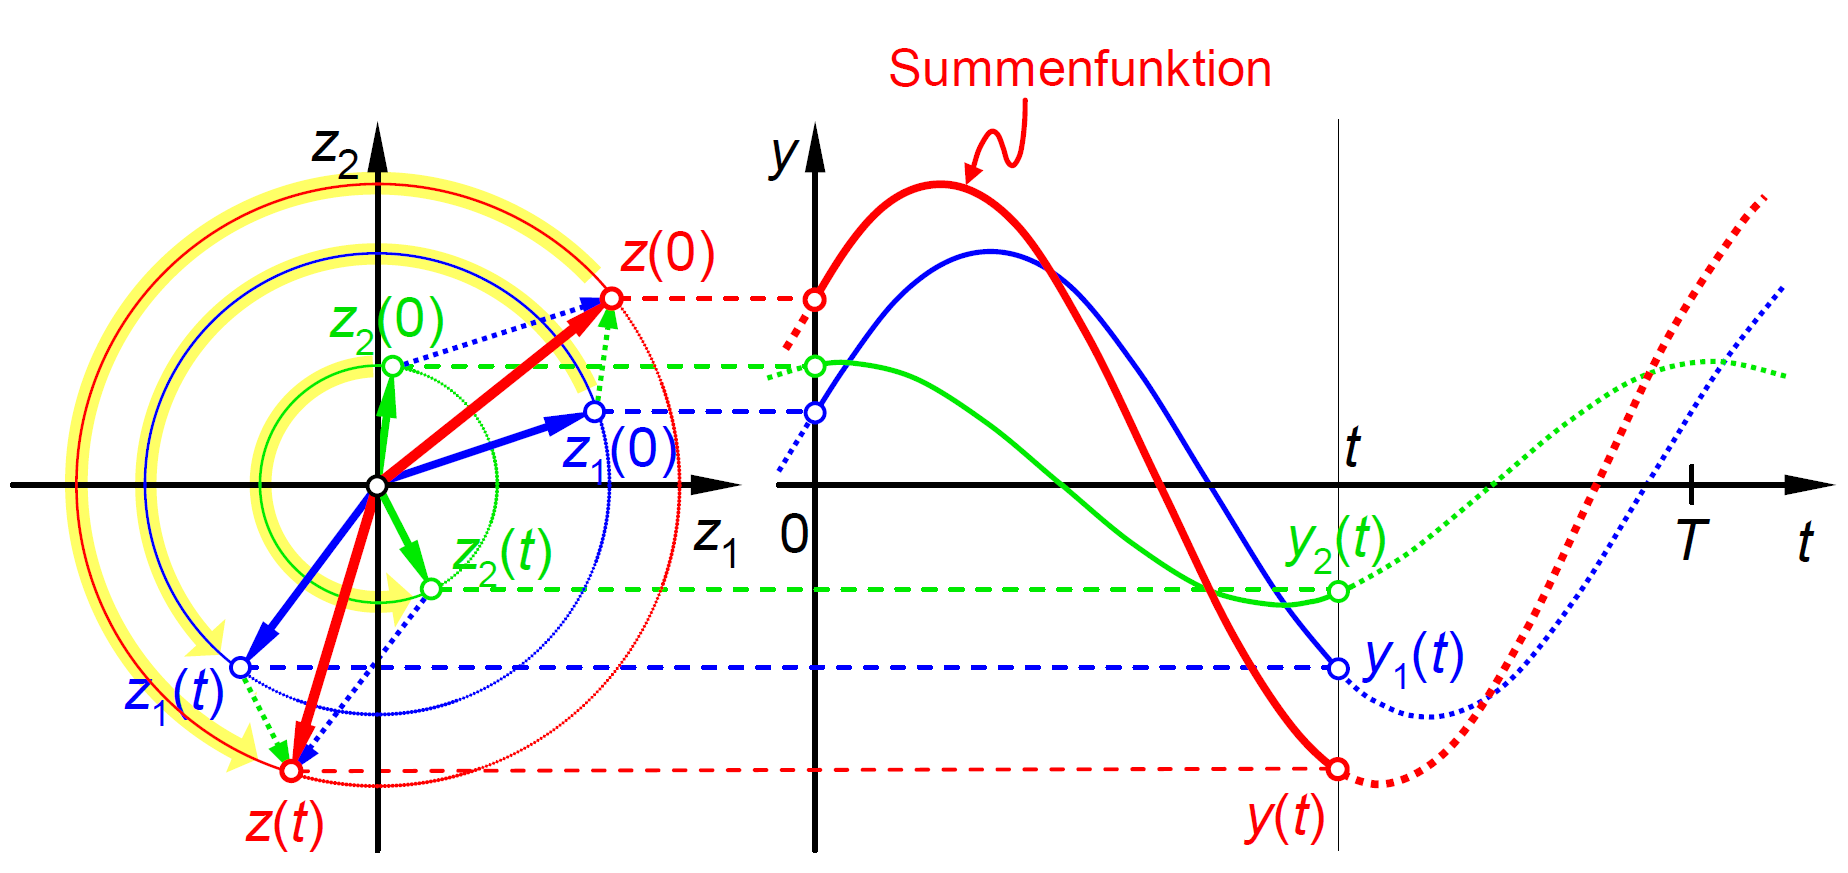
\includegraphics[width=\columnwidth]{images/summe-schwingungen.PNG}

\smallskip

\begin{tabular}{lll@{}}
    Komplexe Amplitude $z_i(0)$ & $z_i(0) = A \cdot \e^{\jimg \varphi_i}$                                                                                       & (zeitunabhängig)  \\
    'Schwingung' / 'Rotation'   & $z(t) = A \cdot \e^{\jimg (\omega t + \varphi)} = \underbrace{A \cdot \e^{\jimg \varphi}}_{z_i(0)} \cdot \e^{\jimg \omega t}$ & (zeitabhängig)
\end{tabular}


\para{Überlagerung gleichfrequenter Schwingungen ($\bm{z(t) = z_1(t) + z_2(t)}$)}
\begin{itemize}
    \item Überlagerung gleichfrequenter Schwingungen entspricht grafischer Addition der
    beiden 'Zeiger' zu jedem Zeitpunkt.
    \item La somma va eseguita solamente usando $\sin \text{o} \cos$, scegliere uno dei
    2 e trasformare l'altro usando prorietà trigonometriche (\ref{chap:trigo-beziehungen})
    \item Per trovare $A$: exp $\rightarrow$ kartesische, eseguire $\sum$, risultato da kartesiche $\rightarrow$ exp
\end{itemize}



\smallskip

\renewcommand{\arraystretch}{1.3}
\begin{tabular}{lll}
    reelle \cor{Amplitude}:   & $A = \vert A_1 \cdot \e^{\jimg \varphi_1} + A_2 \cdot \e^{\jimg \varphi_2} \vert =\cor{a} \cdot e^{\jimg\alpha}$      & (Betrag)  \\
    \cbl{Nullphasenwinkel}    & $\varphi_0 = \arg(A_1 \cdot \e^{\jimg \varphi_1} + A_2 \cdot \e^{\jimg \varphi_2}) =a \cdot e^{\jimg\cbl{\mathbf{\alpha}}}$   & (Winkel)	
\end{tabular}
\renewcommand{\arraystretch}{1}